%------------------------------------------------------------------------------------------------
%
% LaTeX document Tally
%
%------------------------------------------------------------------------------------------------

\documentclass[11pt,a4paper]{article} % weitere Option: twoside

%------------------------------------------------------------------------------------------------

% weitere Pakete laden
        % Kodierung einstellen
\usepackage[ngerman]{babel}
\usepackage[T1]{fontenc}
\usepackage{graphicx}
\usepackage{ngerman}
\usepackage{listings}
\usepackage{color}
\usepackage[utf8x,utf8]{inputenc}
\usepackage{courier}
\usepackage{url}
\usepackage{hyperref}
\usepackage[hyphenbreaks]{breakurl}


\definecolor{dkgreen}{rgb}{0,0.6,0}
\definecolor{gray}{rgb}{0.5,0.5,0.5}
\definecolor{mauve}{rgb}{0.58,0,0.82}

\lstset{numbers=left,
	numberstyle=\tiny,
	numbersep=5pt,
	breaklines=true,
	showstringspaces=false,
	frame=l ,
	xleftmargin=15pt,
	xrightmargin=15pt,
	basicstyle=\ttfamily\scriptsize,
	stepnumber=1,
	keywordstyle=\color{blue},          % keyword style
  	commentstyle=\color{dkgreen},       % comment style
  	stringstyle=\color{mauve}         % string literal style
}






% weitere Formatierung
\frenchspacing                         % Kein zus�tzlichen Abstand nach Punkt (.)
\setlength{\parindent}{0cm}            % keine Einr�ckung bei Beginn eines Absatzes
\setlength{\parskip}{1.5ex plus 0.5ex minus 0.5ex}  % mehr Absatzabstand


%------------------------------------------------------------------------------------------------
%
% 
%
%------------------------------------------------------------------------------------------------


%\pagestyle{empty}                     % keine Kopf- und Fu�zeilen
\pagestyle{plain}                      % nur Seitenzahlen
%\pagestyle{headings}                  % Aktivieren f�r Kopf- und Fu�zeilen



\title{\normalfont\bfseries{Tally\\ digitale Strichliste am Raspberry Pi}\\---}
\author{Nicolai Tegtmeier \\ Dominik Scheffler \\ Philip Frieling \\ Sebastian Reinke}
\date{23.06.2015}


%------------------------------------------------------------------------------------------------

\begin{document}

%------------------------------------------------------------------------------------------------

%\maketitle  % Titel erzeugen, verwendet die Angaben aus \title, \author und \date

%\tableofcontents % Um Inhaltsverzeichnis zu erzeugen

\begin{titlepage}
	\maketitle
	\begin{figure}[h]
	\makebox[\textwidth]{
	
\includegraphics[width=15cm]{TallyLogo.png}}
	\caption{Tally Logo}
	\end{figure}
\end{titlepage}
%------------------------------------------------------------------------------------------------

\tableofcontents
\newpage

\section{Projektvorfeld}
\label{Grundlagen}


\subsection{Kaffeestrichliste bisher}

In kleineren Unternehmen und Arbeitsgruppen gibt es oft einen zentralen Kaffee-/ Getränkeautomaten und Snacks, an denen sich jeder Mitarbeiter bedienen kann. Um die Getränke und Snacks kaufen zu können wird meistens eine Strichliste auf Papier, in der Nähe des Automaten oder der Snacks angebracht, damit sich jeder Mitarbeiter eintragen kann, was er gekauft hat. Diese Liste wird oft zur besseren Verwaltung in eine Datenbank oder Tabelle eingepflegt, damit der Administrator einsehen kann wer wie viel gekauft hat. Hier passiert es jedoch häufig, dass die Strichliste sehr unleserlich wird und es bei der Übertragung in die Datenbank auf den PC zu Fehlern kommt. Außerdem ist diese Methode für den Verantwortlichen sehr zeitaufwendig, da alles per Hand übertragen werden muss.
\par
Um diesem Problem entgegen zu wirken, erarbeiten wir eine neue Methode, um diese Daten 'digital' und somit einfacher speichern zu können.


\section{Rahmenbedingungen}


\subsection{Aufgabe - die neue Kaffeestrichliste}
\label{SchriftAnpassen}

Um eine möglichst energiesparende und handliche Lösung zu finden, sollte die neue Strichliste auf einem Raspberry Pi 2 realisiert werden. Zunächst soll eine passende Benutzeroberfläche für den Raspberry entwickelt werden, damit der Benutzer am Raspberry selber seine Einkäufe verbuchen kann. Dies soll mit Hilfe der integrierten Entwicklungsumgebung 'Qt Creator', die besonders zur Entwicklung von plattformunabhängigen C++ Programmen gedacht ist, entwickelt werden.
\par
Mithilfe eines Webservers, der ebenfalls auf dem Raspberry läuft, soll die Administration von jedem Computer im selben Netzwerk über eine Weboberfläche möglich sein. Hier sollen auch die Benutzer ihre Daten einsehen und ändern können. Dazu wird eine MySQL/ SQLite Datenbank, sowie PHP Unterstützung benötigt. Mittels eines Barcodescanners soll es möglich sein am Raspberry Produkte ein zu scannen.


\section{Ziele des Projekts}
Die neue 'digitale Kaffeestrichliste' wird auf Basis eines Raspberry Pi 2 entwickelt, um die alte Strichliste abzulösen. Dazu wurden folgende zu erreichende Ziele festgelegt:
\subsection{Zielbestimmung}
\label{Ausrichtung}

\subsubsection{Der Benutzer Account}
\"Uber den Benutzer Account soll der Benutzer sich am Raspberry selbst und an der Weboberfläche anmelden können. Am Raspberry selbst können Getränke und Snacks gekauft werden. Mithilfe der Weboberfläche kann der Benutzer Statistiken einsehen und sein Passwort ändern.

\subsubsection{Das Programm}
Das Programm das auf dem Raspberry läuft aktualisiert die Anzahl der Produkte im Lagerbestand automatisch, gibt Meldungen bei zu geringem Warebestand aus und gibt generelle Fehlermeldungen aus.

\subsubsection{Der Administrator Account}
Die Administration mithilfe des Administrator Accounts findet ausschliesslich über die Weboberfläche statt. Hier kann der Administrator Accounts hinzufügen und verwalten, Waren hinzuf\"ugen und verwalten und den Lagerbestand verwalten.

\subsection{Produkteinsatz}
\subsubsection{Anwendungsbereiche}
Mitarbeiter, beziehungsweise die Administratoren, können eine Strichliste 'digital' anlegen. Diese fasst den zu bezahlenden Betrag für die Mitarbeiter zusammen.

\subsubsection{Zielgruppen}
Personengruppen und Unternehmen bei denen Getränke und Snacks privat für alle angeboten und privat bezahlt werden, jedoch Schwierigkeiten mit der Handhabung einer herk\"ommlichen Strichliste haben und den Bestand an Getränken und Snacks erfassen wollen.

\subsubsection{Betriebsbedingungen}
Die Strichliste soll möglichst Wartungsarm und einen niedrigen Stromverbrauch haben. Desweiteren soll sie täglich vierundzwanzig Stunden laufen.

\subsection{Produktumgebung}
Das Produkt kann unabhängig an jedem Ort betrieben werden, solang eine Stromquelle in der Nähe ist.

\subsubsection{Software}
Die einzige Software die vom Benutzer benötigt wird ist ein aktueller Webbrowser.

\subsubsection{Hardware}
Der Benutzer kann mit jedem Internetfähigen Gerät die Weboberfläche erreichen.

\subsubsection{Orgware}
Der Administrator kann die Betriebsparameter konfigurieren.

\subsection{Produktfunktion}
\subsubsection{Benutzerfunktion}
Ein im System registrierter Benutzer kann das System erst nutzen, wenn er angemeldet ist.
Nur ein Administrator kann einen Benutzer anlegen und ihm einen Benutzernamen sowie Passwort zuwesien. Sobald ein Benutzer registriert ist, kann er sich sowohl am Raspberry, als auch an der Weboberfläche anmelden. Dafür benötigt er seinen Benutzernamen und sein Passwort. Abmelden ist bei beiden Oberflächen jederzeit möglich.
\par
Der Administrator kann über die Weboberfläche Produkte hinzufügen,entfernen und deren Details ändern. Benutzer können über Weboberfläche Favoriten einrichten und Statistiken einsehen.
\par
Am Raspberry kann der registrierte und angemeldete Benutzer ein Produkt aus einer Liste wählen oder mithilfe eines Barcodescanners ein Prdoukt einscannen, welches in den Warenkorb gelegt wird. Desweiteren kann er die Anzahl der Produkte erhöhen und seinen gesamten Warenkorb einsehen. Wenn er alle Waren im Warenkorb hat, kann er zur Kasse und die Waren durch einen Klick bezahlen, wodurch sein Konto belastet wird. Ein Abbruch oder das erreichen des Hauptmenüs ist jederzeit möglich.

\subsection{Programmfunktion}
Beim Kauf eines Produktes aktualisiert das Programm automatisch den Warenbestand. Bei geringem Warenbestand wird eine Warnmeldung ausgegeben und bei fehlen des Artikels wird dieser entfernt.

\subsection{Serverfunktion}
Auf dem Raspberry soll ein Apache 2 Server mit PHP Unterstützung laufen.
\subsubsection{Datenbank}
Als Datenbank soll die resourcenschonendere SQLite Datenbank verwendet werden

\subsection{Benutzerschnittstelle}
Die Bedienung des Raspberry erfolgt über einen eingebauten Touchscreen am Raspberry. Außerdem wird ein Barcodescanner installiert um Produkte einscannen zu können.

\newpage


\section{Meilensteine des Projektes}
\label{Meilensteine}

\subsection{Raspberry Pi 2 Model B - Die Hardware mit der passenden Software}
Mit dem Raspberry Pi 2 war schon im Projektvorfeld eine passende Basis für das Projekt gegeben. Der Raspberry Pi 2 besitzt einen Vierkern ARM Cortex-A7 Prozessor mit jeweils 900MHz und einem Gigabyte Arbeitsspeicher. Desweiteren befinden sich vier USB 2.0 Ports, eine 40 GPIO pin Steckerleiste, ein HDMI Anschluss, ein Ethernet Port und ein Micro SD Kartenslot am Raspberry.
	\begin{figure}[h]
	\makebox[\textwidth]{
	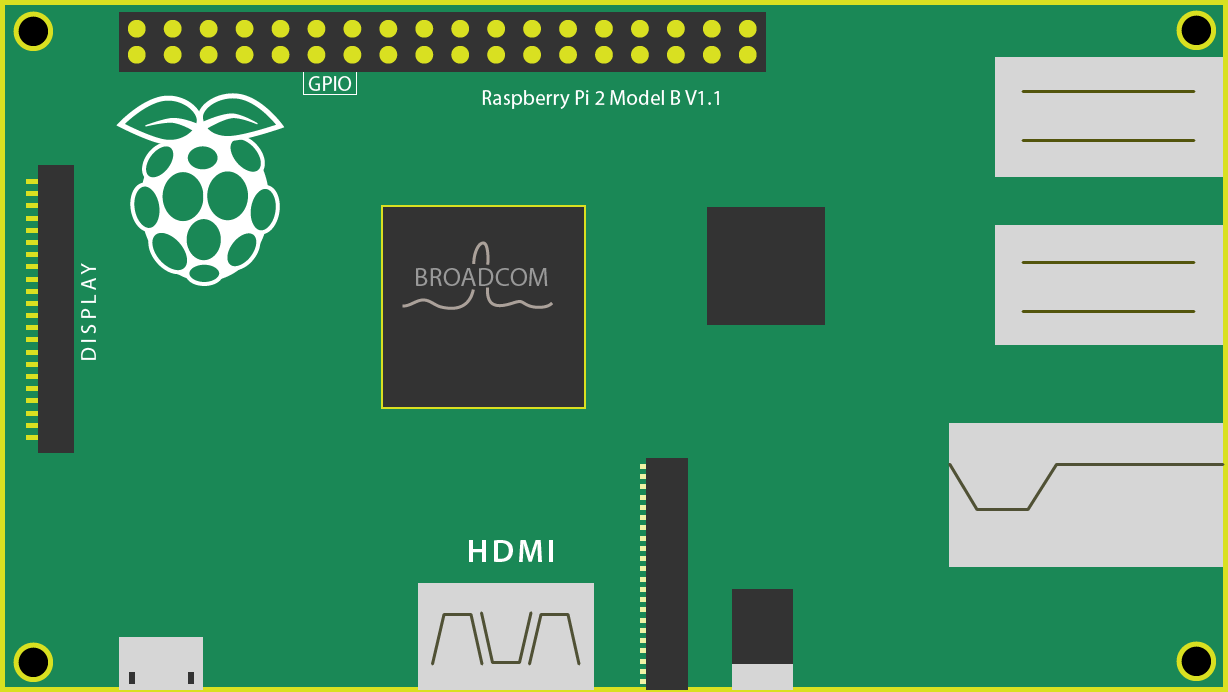
\includegraphics[width=9cm]{RaspberryPi.png}}
	\caption{Der Raspberry Pi 2}
	\end{figure}
\par
Ausser dem Raspberry Pi 2 war zunächst ein 3,5 Zoll Touchscreen der Firma admatec \cite{1} mit dem Namen C-Berry Touch vorhanden, das mittels eines Adapterboards an der GPIO Stiftleiste des Raspberry angesteckt wird. Das Display besitzt eine Auflösung von 320x240 Pixeln, eine LED- Hintergrundbeleuchtung und wird komplett vom Raspberry mit Strom versorgt.
\par
\subsubsection{Betriebssystem und Verbindung zu anderen Rechnern}
Als erster Schritt wurde nach einem passenden Betriebssystem gesucht. Von Anfang an stand fest, dass ein Linuxderivat auf dem Raspberry laufen soll. Hier fiel die Wahl auf das speziell für den Raspberry entwickelte Raspbian.
\par
'Raspbian' ist ein Debianderivat und wurde so optimiert, das es mit den geringen Hardwarespezifikationen zurecht kommt und den ARM-Prozessor des Raspberrys unterstützt. Als Alternative stand eine Ubuntu Version ,speziell für ARM-Prozessoren entwickelt, zu Verfügung, die jedoch noch nicht voll ausgereift ist und somit nicht einwandfrei und resourcenschonend auf dem Raspberry läuft.
\par
 Um die weitere Einrichtung des Raspberrys zu vereinfachen, wurde neben der vorkonfigurierten und installierten SSH Verbindung zur Verwaltung über ein Konsolenprogramm (Windows: Putty), eine freie Implementierung des Remote Desktop Protocols (Windows) für Linux Names 'xrdp' installiert. \cite{2}
\begin{frame}

\begin{lstlisting}
sudo apt-get install xrdp
\end{lstlisting}

\end{frame}
Damit ist eine einfache Remote Desktopverbindung zum Raspberry möglich und die komplette Verwaltung kann über einen Windows, Mac oder Linux Computer erfolgen. 
\par
\subsubsection{Der Webserver}
Als nächstes wurde ein vollständiger Webserver auf dem Raspberry eingerichtet. Hierzu wurde zunächst ein Apache Server der Version 2 installiert
\begin{frame}

\begin{lstlisting}
sudo apt-get install apache2
\end{lstlisting}

\end{frame}
 der über eine hohe Stabilität und Geschwindigkeit verfügt und serverseitig die Skriptsprache PHP unterstützt. Im Anschluss wurde das PHP5 Paket installiert
 \begin{frame}

\begin{lstlisting}
sudo apt-get install php5
\end{lstlisting}

\end{frame}
 um eine volle Unterstützung für die kommende Website zu gewährleisten.
 \par
 PHP ist eine Open Source-Skriptsprache, welche speziell für die Webprogrammierung geeignet ist. Bei einer Anfrage an die Website, wird der PHP-Code auf dem Server ausgeführt und erzeugt eine HTML-Ausgabe die dann letztendlich an den Client gesendet wird.
 \cite{3}
\par
\subsubsection{Qt Creator}
Das Programm an sich, Tally, wird auf einem externen Rechner in Qt programmiert und auf Richtigkeit überprüft, debuggt. Erst dann wird die Version auf GitHub zur Verfügung gestellt und auf den Raspberry geladen.
\par
Damit das Programm auf dem Raspberry lauffähig gemacht werden kann, bzw kompiliert werden kann, muss der Qt Creator\cite{4} samt Qt4 Umgebung installiert werden. Dieser kann dann das gespeichert unkompilierte Programm öffnen und passend für den Raspberry kompilieren.
\par
Das Programm auf einem anderen Computer zu kompilieren entfällt, da das Programm speziell für ARM-Prozessoren kompiliert werden muss. Es gibt zwar die Möglichkeit des Cross-Compilierens, wo man auf einem anderen System als dem gedachten das Programm schreibt aber so kompilieren kann das es auf dem Raspberry läuft. Diese weist aber noch einige Fehler beim kompilieren für den Raspberry auf, so dass ein fehlerfreies programmieren und kompilieren nicht möglich ist.
\par
Für den Qt Creator mit den passenden development Tools führt man folgende Befehle aus
 \begin{frame}

\begin{lstlisting}
sudo apt-get install qtcreator
sudo apt-get install qt4-dev-tools
sudo apt-get install gcc
sudo apt-get install xterm
sudo apt-get install git-core
sudo apt-get install subversion
\end{lstlisting}

\end{frame}
Danach muss man nur noch die passende Toolchain, also den passenden Compiler für den Raspberry, auswählen. Dazu geht man im Qt Creator auf Optionen > build and run > tab tool chains > add und wählt GCC aus. Bei dem Compiler Pfad stellt man folgenden Pfad ein
\begin{frame}

\begin{lstlisting}
/usr/bin/arm-linux-gnueabihf-gcc-4.6 
\end{lstlisting}

\end{frame} 
beim Debugger
  \begin{frame}

\begin{lstlisting}
/usr/bin/gdb
\end{lstlisting}

\end{frame}
Danach nur noch bestätigen und der Qt Creator ist einsatzbereit. Nun kann eine Projektdatei mit der Endung .pro geöffnet und kompiliert werden.
\par
\subsubsection{Die passende Datenbank}
Nun stand die Auswahl des passenden Datenbankverwaltungssystems an. Zur Auswahl standen die Systeme MySQL und SQLite. Bei Recherchen zu den beiden Datenbanken stellte sich schnell heraus das die MySQL Datenbank zwar auf dem Raspberry lauffähig ist aber keine hohe Stabilität besitzt und sehr resourcenlastig auf dem Raspberry läuft. Daher wurde das SQLite Datenbanksystem ausgewählt.
\begin{frame}

\begin{lstlisting}
apt-get install sqlite3
apt-get install php5-sqlite
\end{lstlisting}

\end{frame}
 SQLite ist eine relationale Datenbank und benötigt im Gegensatz zu MySQL keine ständig laufende Software da die Datenbank aus einer einzigen, wenigen Kilobyte grossen, Datei besteht. SQLite  legt Wert auf Geschwindigkeit und Einfachheit.
\par
\subsubsection{Der Touchscreen}
Wie eingangs erwähnt stand neben dem Raspberry der C-Berry Touchscreen von admatec zur Verfügung. \cite{1}
Als erstes wurde der Treiber für den bereitgestellte C-Berry Touchscreen installiert \cite{5}
\begin{frame}

\begin{lstlisting}
wget http://www.airspayce.com/mikem/bcm2835/bcm2835-1.36.tar.gz
tar zxvf bcm2835-1.36.tar.gz
cd bcm2835-1.36
./configure
make
sudo make check
sudo make install
\end{lstlisting}

\end{frame}
und im Anschluss die Beispielsoftware zum anzeigen von Bildern installiert
\begin{frame}

\begin{lstlisting}
wget http://admatec.de/sites/default/files/downloads/C-Berry.tar.gz
tar zxvf C-Berry.tar.gz
cd C-Berry/SW/tft_test
make
sudo ./tft_test
\end{lstlisting}

\end{frame}

Nach ersten Tests mit dem C-Berry Touchscreen wurde bemerkt, dass es nicht als Primäres Display geeignet ist, da vom Desktop ein Screenshot erstellt wird und dieser auf dem Display ausgegeben wird. Starke Verzögerungen im Bildaufbau und eine schlechte Bedienung mithilfe des Touchscreens waren die Folge. Das Display ist dafür gedacht andere Inhalte als den Desktop wiederzugeben, die dann per Touchscreen bedient werden wie zum Beispiel einzelne Buttons.
\par
Damit war der Touchscreen ungeeignet für das Projekt und ein neuer Touchscreen mit besserer Anbindung an den Rapsberry und einer höheren Bildwiederholungsrate musste gesucht werden. Dabei kam die Idee auf, ein 7 Zoll resistives Touchscreen von Pollin \cite{6} zu verwenden, welches durch seine Grösse viel Platz für das Tally Programm bietet und eine sehr gute Touch Bedienung verspricht. Von Vorteil war auch die eigene externe Grafikeinheit die eine hohe Bildwiederholungsrateermöglicht  und ein externer USB- Touchcontroller, der die Bedienung des Touchscreens besser ausführen soll.
\par
Jedoch stellte die externe Stromversorgung ein Problem dar, da man jeweils ein Stromkabel für den Raspberry und eins für das Display benötigt, damit wäre eine Energiesparende Lösung ebenfalls nicht möglich.
\par
Deshalb fiel die Entscheidung zugunsten des 3,5 Zoll Touchscreen 4DPi-35 von 4D System aus.\cite{7} 
\begin{figure}[h]
	\makebox[\textwidth]{
	\includegraphics[width=9cm]{4dpi.png}}
	\caption{Der 4 DPi-35 Touchscreen}
	\end{figure}
Der Touchscreen besitzt eine Auflösung von 480x320 Pixeln und durch die High Speed 48Mhz SPI Verbindung werden hohe und konstante Bildwiederholungsraten ermöglicht.
\newpage
Die Vorteile bei diesem Display waren die kleine Bauform und keine zusätzlich benötigte Stromquelle. Ausserdem wird vom Hersteller direkt ein passender Kernel für Raspbian zur Verfügung gestellt.
\begin{frame}

\begin{lstlisting}
wget http://www.4dsystems.com.au /downloads/4DPi/kernel4dpi_1.3-3_pi2.deb 

sudo dpkg -i kernel4dpi_1.3-3_pi2.deb
\end{lstlisting}

\end{frame}

 Nachdem das erforderliche Paket installiert wurde, musste der Raspberry herunter gefahren und vom Strom getrennt werden. Das Display wird an den GPIO-Ports angebracht und der Raspberry kann wieder mit Strom versorgt und hoch gefahren werden. Danach war ein sofortiger Betrieb möglich da der Raspberry das Display als primäres Display erkennt und direkt auf den Desktop bootet. Dadurch ist kein HDMI Bildschirm mehr notwendig und die Bedienung kann ausschliesslich über den Touchscreen erfolgen.
\par
\subsubsection{Produkte scannen}
Zur vereinfachten Eingabe von Produkten soll ausserdem ein Barcodescanner angebracht werden. Hier sollte entweder ein handelsüblicher Barcodescanner per USB an den Raspberry angeschlossen werden, der Barcode mittels USB Webcam und passender Software oder aber ein Barcodescannermodul an den GPIO's des Raspberry als Lösung dienen.
\par
 Da jedoch das Barcodescannermodul nur mit ca. drei Volt betrieben werden kann, der Raspberry aber ca. fünf Volt an den GPIO's zur Verfügung stellt, fiel diese Möglichkeit weg. Deshalb war eine weitere Möglichkeit, eine Webcam an den Raspberry anzuschliessen und mittels einer Software das Bild auf Barcodes zu untersuchen, wobei es allerdings Probleme mit dem Autofokus der Webcams gab. Damit ein Barcode gelesen werden kann, muss ein Autofokus vorhanden sein, der sich auch passend scharf stellt. Diese Webcams sind allerdings relativ teuer. Die Wahl fiel deshalb auf das Scannen mittels USB Barcodescanner, da dies eine einfacherere Handhabung verspricht und der Barcodescanner direkt als USB Tastatur erkannt wird.
\par
\subsubsection{Wlan für den Raspberry}
Damit am Raspberry nicht immer ein Patchkabel angeschlossen werden muss und nur einen Stromanschluss benötigt wird, wurde der Edimax WLAN USB Stick\cite{8} am Raspberry angeschlossen. Der Edimax WLAN Stick wird automatisch von Raspbian erkannt da schon alle erforderlichen Pakete und Treiber installiert sind. Daher wird der WLAN Stick empfohlen falls man WLAN am Raspberry nutzen möchte. Zunächst wurde der automatische 'Power Saving' Modus abgeschaltet, da der Wlan Stick sonst immer automatisch in den Ruhemodus geht und der Raspberry somit nicht mehr von aussen erreichbar wäre.

Hierzu wurde eine Konfigurationsdatei für den Treiber des WLAN Sticks erstellt.
\begin{frame}

\begin{lstlisting}
sudo nano /etc/modprobe.d/8192cu.conf
\end{lstlisting}

\end{frame}
\par

mit folgendem Inhalt
\begin{frame}

\begin{lstlisting}
options 8192cu rtw_power_mgnt=0 rtw_enusbss=0
\end{lstlisting}

\end{frame}
\par
\par
Um nun eine Verbindung mit dem Wlan herzustellen wurde die folgende Datei
\begin{frame}

\begin{lstlisting}
sudo nano /etc/network/interfaces
\end{lstlisting}

\end{frame}

um folgenden Inhalt ergänzt
\begin{frame}

\begin{lstlisting}
auto lo
iface lo inet loopback
iface eth0 inet dhcp

auto wlan0
allow-hotplug wlan0
iface wlan0 inet dhcp
wpa-ap-scan 1
wpa-scan-ssid 1
wpa-ssid "WLAN-NAME"
wpa-psk "WLAN-PASSWORT"

\end{lstlisting}

\end{frame}

damit eine Verbindung mit dem WLAN Netz hergestellt werden kann.
Anschliessend muss nur noch per
\begin{frame}

\begin{lstlisting}
sudo service networking restart
\end{lstlisting}

\end{frame}
der Netzwerkdienst neu gestartet werden und eine Verbindung mit dem angegebenen WLAN Netz wird hergestellt.
\par
Da diese Möglichkeit jedoch relativ umständlich ist und Linux Kenntnisse erfordert, wird in das Tally Programm eine einfache WLAN Konfiguration eingebaut, in der man den WLAN-Namen und das WLAN-Passwort eingeben kann um sich mit dem WLAN-Netz zu verbinden.

\subsubsection{angepasster Bootscreen}
Während eines Meetings kam die Idee auf, den Bootscreen zu verändern und ein eigenes Bild während des hochfahrens anzuzeigen. Dazu wird eine weitere Software benötigt, der 'Frame Buffer Imageviewer', der ein Bild in den Speicherbuffer lädt, welches während des Hochfahrens angezeigt werden kann. \cite{9}

\begin{figure}[h]
	\makebox[\textwidth]{
	
\includegraphics[width=9cm]{bootscreen.png}}
	\caption{Bootlogo}
	\end{figure}

\begin{frame}

\begin{lstlisting}
sudo apt-get install fbi
\end{lstlisting}

\end{frame}

Danach muss ein passendes Skript geschrieben werden welches das Bild beim booten anzeigt.
\begin{frame}

\begin{lstlisting}
sudo nano asplashscreen
\end{lstlisting}

\end{frame}
\newpage
mit folgendem Inhalt
\begin{frame}

\begin{lstlisting}
#! /bin/sh
### BEGIN INIT INFO
# Provides:          asplashscreen
# Required-Start:
# Required-Stop:
# Should-Start:      
# Default-Start:     S
# Default-Stop:
# Short-Description: Show custom splashscreen
# Description:       Show custom splashscreen
### END INIT INFO
 
do_start () {
 
    /usr/bin/fbi -T 1 -noverbose -a /etc/splash.png    
    exit 0
}
 
case "$1" in
  start|"")
    do_start
    ;;
  restart|reload|force-reload)
    echo "Error: argument '$1' not supported" >&2
    exit 3
    ;;
  stop)
    # No-op
    ;;
  status)
    exit 0
    ;;
  *)
    echo "Usage: asplashscreen [start|stop]" >&2
    exit 3
    ;;
esac
 
:
\end{lstlisting}

\end{frame}

Dieses Skript wird nun in den passenden Ordner verschoben damit es beim Start ausgeführt werden kann
\begin{frame}

\begin{lstlisting}
sudo mv asplashscreen /etc/init.d/asplashscreen
\end{lstlisting}
\end{frame}

Als letztes wird das Skript für den Raspberry ausführbar gemacht und als Bootscript registriert
\begin{frame}

\begin{lstlisting}
sudo chmod a+x /etc/init.d/asplashscreen
sudo insserv /etc/init.d/asplashscreen
\end{lstlisting}
\end{frame}

Nun wird w\''ahrend des Bootvorgangs das Tally Logo angezeigt.
\newpage

\subsubsection{Backups einrichten und versenden per Mail}
Als m\"ogliche Backupvarianten standen ein komplettes Backup der Speicherkarte des Raspberrys oder ein Backup der Datenbank zur Wahl.
\par
Der Entschluss fiel auf ein Backup der Datenbank, da diese auch per Mail an den jeweiligen Administrator geschickt werden soll. Dazu wird Rsync verwendet, das mit folgendem Befehl installiert wird:
\begin{frame}

\begin{lstlisting}
sudo apt-get install rsync
\end{lstlisting}
\end{frame}
 Rsync ist ein Programm das Dateien oder Ordner in verschiedenen Pfaden speichern kann. Dazu überprüft es zunächst ob die zu kopierende Datei geändert wurde oder nicht, wodurch ein unnützes kopieren von Daten unterbunden wird.
\par
Damit die backups autmatisch und täglich erstellt werden, wird ein cronjob hinzugefügt. Cron-Daemon ist ein Dienst um Skripte oder Programme zu einer bestimmten Zeit starten zu lassen, ohne diese aktiv aufrufen zu müssen. Der Befehl dazu wird in der zugehörigen Tabelle, der crontab, gespeichert. Zunächst wird die Tabelle crontab mit dem editier-Befehl geöffnet
\begin{frame}

\begin{lstlisting}
sudo crontab -e
\end{lstlisting}
\end{frame}

Hier wird folgende Zeile eingefügt
\begin{frame}

\begin{lstlisting}
15 22 * * * rsync -av --delete /var/www/sqlite/database.sqlite  /home/pi/Tally/sicherung
\end{lstlisting}
\end{frame}
Dadurch wird das Programm jeden Tag um 22:15Uhr aufgerufen und die Datenabank von /var/www/sqlite nach /home/pi/Tally/sicherung  kopiert. Hier wurde die erste Stelle auf 15 gesetzt welche die Minuten Angabe ist, die zweite auf 22 für die Stunden Angaben. Die dritte Stelle gibt an, an welchem Tag das Skript/Programm ausgeführt werden soll, die vierte an welchem Monat und die fünfte an welchem Wochentag. Da rsync jeden Tag ausgeführt werden soll werden nur die ersten beiden Stellen angegeben.
\par
Diese Datei soll nun auch täglich, nach dem erstellen des Backups, an den Admin per mail gesendet.
Dafür wird das Programm sendEmail und zwei Perl- Libraries installiert.
\begin{frame}

\begin{lstlisting}
sudo apt-get install sendemail libio-socket-ssl-perl libnet-ssleay-perl
\end{lstlisting}
\end{frame}
SendEmail hat den Vorteil das kein Mailserver auf dem Raspberry installiert werden muss und der Raspberry als ein eigener 'sende Client' erkannt wird und nur die Zugangsdaten zum SMTP-Server des Email Accounts über den gesendet werden soll hinterlegt werden müssen. Die beiden Perl- Libraries dienen dazu damit eine verschlüsselte Verbindung per TLS zum Mailserver aufgebaut werden kann.
\par
Zum automatischen versenden der Mails wird folgendes Skript erstellt, das vielfach für den Raspberry verwendet wird. Im Code findet sich der Name des Autors \cite{10}
\begin{frame}

\begin{lstlisting}
sudo nano /usr/local/bin/mailnotify.sh
\end{lstlisting}
\end{frame}

Das Skript sieht wie folgt aus
\begin{frame}

\begin{lstlisting}
###########################################################################
                                                                     												  
              Sending E-Mail notification with sendEmail              									 
                                                                      											 
 Creation:    15.08.2013                                              										 
 Last Update: 20.10.2013                                               										 
                                                                       											
 Copyright (c) 2013 by Georg Kainzbauer <http://www.gtkdb.de>          							
                                                                      											 
 This program is free software; you can redistribute it and/or modify 								 
 it under the terms of the GNU General Public License as published by								  
 the Free Software Foundation; either version 2 of the License, or    								 
 (at your option) any later version.                                   									
                                                                       											
###########################################################################
#!/bin/bash

# Sender of the mail
SENDER="absender@domain.de"

# Recipient of the mail
RECIPIENT="empfaenger@domain.de"

# SMTP server
SMTPSERVER="smtp.domain.de"

# User name on the SMTP server
SMTPUSERNAME="MeinMailAccount"

# Password on the SMTP server
SMTPPASSWORD="MeinMailPasswort"

# Enable TLS for the SMTP connection
USETLS=1

###################################################################
# NORMALLY THERE IS NO NEED TO CHANGE ANYTHING BELOW THIS COMMENT #
###################################################################

# Use first argument as mail subject
if [ -n "$1" ]; then
  SUBJECT="$1"
else
  # No subject specified
  SUBJECT=""
fi

# Use second argument as mail body
if [ -n "$2" ]; then
  BODY="$2"
else
  # No mail body specified
  BODY=""
fi

# Generate the options list for sendEmail
OPTIONS=""

if [ -n "${SMTPSERVER}" ]; then
  OPTIONS="${OPTIONS} -s ${SMTPSERVER}"
fi

if [ -n "${SMTPUSERNAME}" ]; then
  OPTIONS="${OPTIONS} -xu ${SMTPUSERNAME}"
fi

if [ -n "${SMTPPASSWORD}" ]; then
  OPTIONS="${OPTIONS} -xp ${SMTPPASSWORD}"
fi

if [ -n "${USETLS}" ]; then
  if [ ${USETLS} == 1 ]; then
    OPTIONS="${OPTIONS} -o tls=yes"
  else
    OPTIONS="${OPTIONS} -o tls=no"
  fi
fi

# Send the mail with sendEmail
sendEmail -f ${SENDER} -t ${RECIPIENT} -u "${SUBJECT}" -m "${BODY}" ${OPTIONS}

exit 0
\end{lstlisting}
\end{frame}

Zu editieren sind folgende Punkte:
\begin{frame}

\begin{lstlisting}
# Sender of the mail
SENDER="absender@domain.de"

# Recipient of the mail
RECIPIENT="empfaenger@domain.de"

# SMTP server
SMTPSERVER="smtp.domain.de"

# User name on the SMTP server
SMTPUSERNAME="MeinMailAccount"

# Password on the SMTP server
SMTPPASSWORD="MeinMailPasswort"
\end{lstlisting}
\end{frame}
Hier müssen nur noch die sende Email Adresse, Sender of the mail, der Empfänger der Mail, Recipient of the mail und der SMTP Server mit dazugehörigen Benutzername und Passwort angegeben werden.
Danach muss das Skript ausführbar gemacht werden
\begin{frame}

\begin{lstlisting}
sudo chmod +x /usr/local/bin/mailnotify.sh
\end{lstlisting}
\end{frame}

Im Anschluss kann die erste Email versendet werden
\begin{frame}

\begin{lstlisting}
mailnotify.sh "Test" "Dies ist eine Testnachricht."

\end{lstlisting}
\end{frame}
\newpage
Damit wird das Skript aufgerufen, wobei der text in den ersten Anführungszeichen den Betreff, und der Text in den zweite Anführungszeichen den Inhalt der Email.
Hierbei kam es jedoch zu folgendem Fehler
\begin{frame}

\begin{lstlisting}
invalid SSL_version specified at /usr/share/perl5/IO/Socket/SSL.pm line 332

\end{lstlisting}
\end{frame}

Dieser Fehler entsteht da die dazugehörige SSL konfiguration einen kleinen Fehler enthählt.
Folgende Datei muss aufgerufen werden
\begin{frame}

\begin{lstlisting}
sudo nano /usr/share/perl5/IO/Socket/SSL.pm

\end{lstlisting}
\end{frame}

und in Zeile 1490 muss folgender Inhalt
\begin{frame}

\begin{lstlisting}
m{^(!?)(?:(SSL(?:v2|v3|v23|v2/3))|(TLSv1[12]?))$}i

\end{lstlisting}
\end{frame}

durch
\begin{frame}

\begin{lstlisting}
m{^(!?)(?:(SSL(?:v2|v3|v23|v2/3))|(TLSv1[12]?))}i

\end{lstlisting}
\end{frame}

ersetzt werden.Nur das Dollar Zeichen am Schluss muss entfernt werden. Anschliessend können Emails versendet werden
\begin{frame}

\begin{lstlisting}
mailnotify.sh "Test" "Dies ist eine Testnachricht."
Jul 15 16:32:30 raspberrypi sendEmail[4163]: Email was sent successfully!

\end{lstlisting}
\end{frame}
\par
Damit auch Anhänge mit versandt werden können muss lediglich das Skript etwas verändert werden.
Hinzu kommt folgender Ausdruck. \cite{11}
\begin{frame}

\begin{lstlisting}
# Use third argument as attachment
if [ -n "$3" ]; then
  ATTACHMENT="$3"
else
  # No attachment specified
  ATTACHMENT=""
fi

\end{lstlisting}
\end{frame}
\newpage
Somit sieht das Skript wie folgt aus
\begin{frame}

\begin{lstlisting}
#!/bin/bash

# Sender of the mail
SENDER="absender@domain.de"

# Recipient of the mail
RECIPIENT="empfaenger@domain.de"

# SMTP server
SMTPSERVER="smtp.domain.de"

# User name on the SMTP server
SMTPUSERNAME="MeinMailAccount"

# Password on the SMTP server
SMTPPASSWORD="MeinMailPasswort"

# Enable TLS for the SMTP connection
USETLS=1

###################################################################
# NORMALLY THERE IS NO NEED TO CHANGE ANYTHING BELOW THIS COMMENT #
###################################################################

# Use first argument as mail subject
if [ -n "$1" ]; then
  SUBJECT="$1"
else
  # No subject specified
  SUBJECT=""
fi

# Use second argument as mail body
if [ -n "$2" ]; then
  BODY="$2"
else
  # No mail body specified
  BODY=""
fi

# Use third argument as attachment
if [ -n "$3" ]; then
  ATTACHMENT="$3"
else
  # No attachment specified
  ATTACHMENT=""
fi

# Generate the options list for sendEmail
OPTIONS=""

if [ -n "${SMTPSERVER}" ]; then
  OPTIONS="${OPTIONS} -s ${SMTPSERVER}"
fi

if [ -n "${SMTPUSERNAME}" ]; then
  OPTIONS="${OPTIONS} -xu ${SMTPUSERNAME}"
fi

if [ -n "${SMTPPASSWORD}" ]; then
  OPTIONS="${OPTIONS} -xp ${SMTPPASSWORD}"
fi

if [ -n "${USETLS}" ]; then
  if [ ${USETLS} == 1 ]; then
    OPTIONS="${OPTIONS} -o tls=yes"
  else
    OPTIONS="${OPTIONS} -o tls=no"
  fi
fi

if [ -n "${ATTACHMENT}" ]; then
  OPTIONS="${OPTIONS} -a ${ATTACHMENT}"
fi

# Send the mail with sendEmail
sendEmail -f ${SENDER} -t ${RECIPIENT} -u "${SUBJECT}" -m "${BODY}" ${OPTIONS}

exit 0
\end{lstlisting}
\end{frame}
Und in unserem Fall
\begin{frame}

\begin{lstlisting}
###########################################################################
                                                                   
              Sending E-Mail notification with sendEmail               
                                                                       
 Creation:    15.08.2013                                              
 Last Update: 06.04.2015                                               
 
 Copyright (c) 2013-2015 by Georg Kainzbauer <http://www.gtkdb.de>     
                                                                       
 This program is free software; you can redistribute it and/or modify  
 it under the terms of the GNU General Public License as published by  
 the Free Software Foundation; either version 2 of the License, or     
 (at your option) any later version.                                   
                                                                       
###########################################################################
#!/bin/bash

# Sender of the mail
SENDER="tallyupb@gmail.com"

# Recipient of the mail
RECIPIENT="tallyupb@gmail.com"

# SMTP server
SMTPSERVER="smtp.gmail.com"

# User name on the SMTP server
SMTPUSERNAME="tallyupb@gmail.com"

# Password on the SMTP server
SMTPPASSWORD="kaffee123"

# Enable TLS for the SMTP connection
USETLS=1

###################################################################
# NORMALLY THERE IS NO NEED TO CHANGE ANYTHING BELOW THIS COMMENT #
###################################################################

# Use first argument as mail subject
if [ -n "$1" ]; then
  SUBJECT="$1"
else
  # No subject specified
  SUBJECT=""
fi

# Use second argument as mail body
if [ -n "$2" ]; then
  BODY="$2"
else
  # No mail body specified
  BODY=""
fi

# Use third argument as attachment
if [ -n "$3" ]; then
 ATTACHMENT="$3"
else
  # No attachment specified
  ATTACHMENT=""
fi

# Generate the options list for sendEmail
OPTIONS=""

if [ -n "${SMTPSERVER}" ]; then
  OPTIONS="${OPTIONS} -s ${SMTPSERVER}"
fi

if [ -n "${SMTPUSERNAME}" ]; then
  OPTIONS="${OPTIONS} -xu ${SMTPUSERNAME}"
fi

if [ -n "${SMTPPASSWORD}" ]; then
  OPTIONS="${OPTIONS} -xp ${SMTPPASSWORD}"
fi

if [ -n "${USETLS}" ]; then
  if [ ${USETLS} == 1 ]; then
    OPTIONS="${OPTIONS} -o tls=yes"
  else
    OPTIONS="${OPTIONS} -o tls=no"
  fi
fi

if [ -n "${ATTACHMENT}" ]; then
  OPTIONS="${OPTIONS} -a ${ATTACHMENT}"
fi

# Send the mail with sendEmail
sendEmail -f ${SENDER} -t ${RECIPIENT} -u "${SUBJECT}" -m "${BODY}" ${OPTIONS}

exit 0
\end{lstlisting}
\end{frame}
Im Befehl zum senden wird nun ein drittes Argument hinzugefügt das den Pfad mit der Datei die zu versenden ist enth\"alt.
\begin{frame}

\begin{lstlisting}
mailnotify.sh "Test" "Dies ist eine Testnachricht." anhang.txt

\end{lstlisting}
\end{frame}
\par
Nun muss dieses Skript wieder in die crontab eingefügt werden damit es täglich zu einer bestimmten Zeit ausgeführt wird
\begin{frame}

\begin{lstlisting}
sudo crontab -e

\end{lstlisting}
\end{frame}
hinzugefügt wird
\begin{frame}

\begin{lstlisting}
45 23 * * * /bin/bash /usr/local/bin/mailnotify.sh "Sicherung Tally Datenbank" "Dies ist eine automatische Sicherungsmail der Tally Datenbank" /home/pi/Tally/sicherung/database.sqlite

\end{lstlisting}
\end{frame}
Damit wird das Skript mailnotify.sh um 23:45Uhr gestartet und eine Email mit dem Betreff `Sicherung Tally Datenbank', dem Inhalt der Mail `Dies ist eine automatische Sicherungsmail der Tally Datenbank' und dem Dateianhang `/home/pi/Tally/sicherung/database.sqlite' gesendet.

\subsubsection{Tally autostarten}
Damit nach dem starten des Raspberry Pi direkt das Tally Programm geladen wird musste der Autostart für das Programm konfiguriert werden.
\par
Die erste Idee war das Programm per cronjob nach jedem neuen hochfahren zu starten. Dafür musste zunächst ein kleines Skript geschrieben werden das das Programm startet, welches dann in einer crontab nach jedem hochfahren ausgeführt wird.
\begin{frame}

\begin{lstlisting}
sudo nano /etc/init.d/NameDesSkripts
\end{lstlisting}
\end{frame}
\newpage
Mit folgendem Inhalt
\begin{frame}

\begin{lstlisting}
#! /bin/sh
### BEGIN INIT INFO
# Provides: NAME DES PROGRAMMES
# Required-Start: $syslog
# Required-Stop: $syslog
# Default-Start: 2 3 4 5
# Default-Stop: 0 1 6
# Short-Description:
# Description:
### END INIT INFO
 
case "$1" in
  start)
    echo "NAME DES PROGRAMMES wird gestartet"
    # Starte Programm
    /pfad/des/programmes
    ;;
  stop)
    echo "NAME DES PROGRAMMES wird beendet"
    # Beende Programm
    killall noip2
    ;;
  *)
    echo "Benutzt: /pfad/des/programmes {start|stop}"
    exit 1
    ;;
esac
 
exit 0
\end{lstlisting}
\end{frame}

Danach wird das Skript ausführbar gemacht
\begin{frame}

\begin{lstlisting}
sudo chmod 755 /etc/init.d/NameDesSkripts
\end{lstlisting}
\end{frame}
Um zu testen ob das Skript auch richtig funktioniert wird es mit folgendem Befehl aufgerufen
\begin{frame}

\begin{lstlisting}
sudo /etc/init.d/NameDesSkripts start
\end{lstlisting}
\end{frame}

und wieder gestoppt
\begin{frame}

\begin{lstlisting}
sudo /etc/init.d/NameDesSkripts stop
\end{lstlisting}
\end{frame}

Damit der Raspberry das Skript beim booten lädt wird noch folgender Befehl ausgeführt der das Programm in den passenden Runlevel bringt
\begin{frame}

\begin{lstlisting}
sudo update-rc.d NameDesSkripts defaults
\end{lstlisting}
\end{frame}
\par

Als nächstes soll das Skript durch einen im crontab hinterlegten Befehl jedes mal beim starten des Raspberrys ausgeführt werden
\begin{frame}

\begin{lstlisting}
sudo crontab -e
\end{lstlisting}
\end{frame}
\newpage
Dazu wurde folgende zeile eingefügt
\begin{frame}

\begin{lstlisting}
@reboot \bin\bash /etc/init.d/NameDesSkripts
\end{lstlisting}
\end{frame}
Das '@reboot' steht für das ausführen der Datei nach jedem neuen hochfahren des Raspberry. Jedoch startete das Programm nach dem hoch fahren des Raspberrys nicht. Erst als die Konsole geöffnet wurde startete das Skript und somit das Programm.
\par
Die beschriebene Methode war lediglich dafür gedacht Programme auszuführen die keine GUI benötigen. Alle Programme die autostarten sollen und eine GUI benötigen müssen über die globale LXDE (Lightweight X11 Desktop Environment) Autostart funktion gestartet werden. \cite{12}
Dazu erstellt man in folgendem Pfad
\begin{frame}

\begin{lstlisting}
/etc/xdg/autostart/
\end{lstlisting}
\end{frame}
eine Datei die wie folgt lauten muss 'NamedesProgramm.desktop'. Wichtig ist das die Datei auf `.desktop' endet da sonst das Programm nicht nach dem hochfahren gestartet wird.
\begin{frame}

\begin{lstlisting}
[Desktop Entry]
Name=NamedesProgramm
Comment=
Exec=PfaddesProgramm -forever -rfbport 5900 -rfbauth ~/.vnc/x11vnc.pass -o ~/.vnc/x11vnc.log -display :0
Terminal=false
Type=Application
\end{lstlisting}
\end{frame}

Diese Datei wieder ausführbar machen
\begin{frame}

\begin{lstlisting}
chmod +x x11vnc.desktop
\end{lstlisting}
\end{frame}
Und das gewünschte Programm startet nachdem die GUI geladen ist.

\newpage

\subsection{QT Creator - Das Tally Programm}
Als Programmierumgebung, für den Raspberry Pi 2, wurde Qt gewählt. \cite{13}
Qt ist eine Klassenbibliothek in C++, vereinfacht die Programmierung für graphische Benutzeroberflächen und bietet zahlreiche weitere Funktionen an.
Wir arbeiten mit der Version 4.8.1 von Qt, da neuere Versionen noch nicht mit dem Raspberry Pi 2 kompatibel ist.
Als Debugger haben wir GNU gdb 7.8 und MinGW 4.9.1 als Compiler gewählt.
\par
Programmiert wird hauptsächlich auf unseren eigenen PCs, da diese schneller debuggen können.
Darüber hinaus musste der Raspberry PI 2 noch konfiguriert werden, wie in 4.1 beschrieben, wodurch ein zeitgleiches arbeiten erschwert wäre.
Es wurde sich darauf geeinigt das Programm zu Demonstrationszwecke, während den Teammeetings, auf dem Raspberry PI 2 laufen zu lassen.
Zum Ende des Projekts, sobald die Konfiguration beendet ist, sollten wir denn Raspberry PI 2 bekommen um die Benutzeroberfläche letztendlich anpassen zu können.
\par
\subsubsection{Die Benutzeroberfläche}
Als erstes haben wir erste Grundzüge der Benutzeroberfläche thematisiert. Letztendlich haben wir die GUI herausgearbeitet, welche in dem Plichtenheft zu sehen ist.[Information]
Außerdem wurden mehrere Strukturen für das Hauptprogramm besprochen und haben uns auf einen Automaten geeinigt. Näheres dazu findet sich in dem Unterpunkt Aufbau des Programmes.
\par
Daraufhin wurde sich in Qt eingelesen und die ersten Funktionen für den Login-Screen programmiert. \cite{14} \cite{15}
Wie bereits in Abschnitt 4.1 erklärt, wurde entschieden das Display zu wechseln.
Außerdem ist uns Aufgefallen das sehr viele Klicks gebraucht werden um eine Kaufvorgang abzuschließen, was benutzerunfreundlich ist.
Aus diesen beiden Gründen wurde die komplette Benutzeroberfläche überarbeitet.
\par
Die Knopfgröße und die Schriftgröße mussten vergrößert werden als auch das Knöpfe, aufgrund Platzmangels, weggelassen werden mussten.
Die Screens sollten aber erst beim Programmieren festgelegt werden um evtl. Hürden zu meistern.
Außerdem wussten wir zu diesem Zeitpunkt noch nicht, welches Display für den Raspberry Pi 2 gewählt wird.
\par
\subsubsection{Datenbank und Tally}
Nach dem die ersten Funktionen des Login-Screens und des Passwort-Screen implementiert wurden, wurde begonnen die Datenbank mit einzuarbeiten.
Aus Abschnitt 4.1 geht heraus, dass wir uns für SQLite entschieden haben. Um auf diese zuzugreifen, mussten wir uns zunächst darauf einigen, welche Tabellen angelegt werden und womit diese befüllt werden.
\par
Nachdem wir uns auf die Datenbank geeinigt haben, wurde diese in das Programm implementiert.
Zu diesem Zeitpunkt wurde noch nicht mit einer eindeutigen ID jedes Benutzer gearbeitet sondern mit seinem Namen, was später zu Komplikationen führen würde.
Zeitgleich zum Login-Screen und dem Passwort-Screen wurden alle, die bis zu diesem Zeitpunkt erarbeitete Screen oberflächlich implementiert.
\par
So konnten man zu diesem Zeitpunkt sich anmelden, (die Daten dafür wurden aus der Datenbank genommen) und konnte sich über alle Screens klicken, auch wenn die meisten keine Funktionen hatten.
\par
Nachdem das Grundgerüst des Programmes stand, wurde um die Kauffunktion implementieren zu können, die ID der eingeloggten Person global im Programm bekannt gemacht werden.
Dies haben wird entweder über get-Funktionen realisiert oder beim Erzeugen eines neuen Screens mitgegeben.
Daraufhin konnten die restlichen Funktionen implementieren werden.
\par
Als erstes wurden die Liste implementiert in welche alle kaufbaren Artikel aufgelistet werden.
Die Information über die Artikel konnten über die Datenbank eingelesen werden.
Nachdem sich die Listen mit Artikeln befüllten, wurde mit dem Hauptaspekt des Programmes begonnen, dem Kaufvorgang.
\par
Für den Kaufvorgang ist hauptsächlich das Shoppingcart verantwortlich. Sobald ein Artikel dort liegt, wird es immer auf dem rechten Teil des Bildschirmes angezeigt.
Außerdem ist es dafür verantwortlich, dass wenn Artikel gekauft werden, der Kaufvorgang korrekt abgeschlossen wird.
Dies bedeutet vor allem, dass die Datenbank mit neuen Informationen gefüllt wird. Einerseits wird die Anzahl der entsprechenden Artikel geändert und das Konto des Käufers belastet.
Dies bürgte eine große Hürde. Das Problem mit der Synchronität des Shoppingcart über den gesamten Einkauf.
\par
Jedes Mal wenn der Zustannd gewechselt wurde(siehe Aufbau des Programmes), wurde das Shoppingcart gelöscht und damit auch der Inhalt.
Das Shoppingcart ist ein eigenständiges Teil Programme und somit sollte es unabhängig sein, wenn sich der Zustand des Programmes ändert.
Da wir allerdings keinen Weg gefunden haben ein Widget auf mehrere Widgets angezeigt zu haben, konnten wir das Problem auch nicht anders lösen. Das Soppingcart erstellt nun vor jedem löschen eine Liste mit seinen Items, welche dem neu erzeugten Shoppigcart gegeben wird.
\par
Bis zu diesem Zeitpunkt wurde das Programm fast ausschließlich auf einem PC programmiert, debugt und auch die Größen wurden auf diesen angepasst, wie bereits anfangs erwähnt.
Deswegen war der nächste Schritt die Benutzer Oberfläche, mit dem Raspberry PI 2 und dem neuen Display, anzupassen.
Zusätzlich wurde auch der Barcode Scanner implementiert, was kein Problem dargestellt hat, da sich das Signal des Barcode Scanners verhält wie ein Tastendruck mit der Tastatur. Qt stellt für solche Signale bereits Funktionen.
\par
Somit war das Programm so gut wie fertig. Es fehlten nur noch ein paar kleine Funktionen und vor allem musste noch eventuelle Bugs entfernt werden.
Alle Funktionen des Programmes wurden nicht während dieses Abschnittes erfasst, da dies den Umfang dieser Dokumentation sprengen würde.
Alle wichtigen Funktionen wurde erwähnt und gegebenenfalls erläutert, darüber hinuas werden noch welche in dem Unterpunkt Aufbau des Programmes näheres erklärt.
\par


\subsubsection{Aufbau des Programmes}
Das Programm wurde in 13 Klassen und einer main unterteilt.Im folgendem werden die einzelnen Klassen erläutert.
Allgemein läuft das Programm nach einem Automaten ab. Der Bildschirm wurde in zwei Bereiche unterteilt, wodurch nicht bei jedem Zustandswechsel der komplette Bildschirm neu geladen werden muss, sondern nur der betreffende Teil.
Dadurch Teilen wir den Bildschirm in die Kopfzeile und der Automatenbereich. Näheres dazu wird in den dementsprechenden Klassen erläutert.
main.cpp :
	Die main.cpp ist verantwortlich für den Ablauf des Programmes. Die Struktur dafür ist aufgebaut wie ein Mealy-Automat.Die Zustände geben an welcher Bildschirm gerade angezeigt wird. Die Übergänge sind die Exitcodes.
	Die Ausgaben der Kanten sind jeweils der Screen-Wechsel, welcher nicht im Automaten abgebildet ist.
	
	\begin{figure}[h]
	\makebox[\textwidth]{
	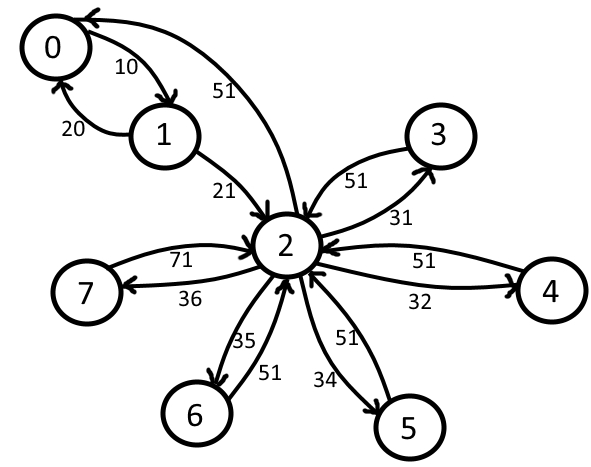
\includegraphics[width=9cm]{automat.png}}
	\caption{MEALEY}
	\end{figure}
	
	Exitcodes erlaubt es Programmen bei bestimmten Events(z.B. ein Knopf wurde geklickt) wieder zurück in die main.cpp zu gelangen.
	 -->mainWindowPointer->exit(21); 
	Es wird Anfangs die Ip ermittelt und diese auf einem eigenen Screen angezeigt.
	-->QTcpSocket socket;
    QString ip;
\begin{frame}

\begin{lstlisting}
    socket.connectToHost(`8.8.8.8', 53); // google DNS, or something else reliable
    if (socket.waitForConnected()) {
        ip = socket.localAddress().toString();
    } else {
        ip = socket.errorString();
    }
    w.showIpScreen(ip);
\end{lstlisting}
\end{frame}
\par
\paragraph{Zustände:} $\;$ \\
		0 : Es wird der Login-Screen auf dem Bildschirm gezeigt.
			Exitcode: 
\begin{enumerate}
			\item	10 : Es wurde der Benutzer gewählt und möchte sich nun mit dem Account anmelden.
			\item	!10 \& !100 \& !34 : Das Programm beendet sich.
\end{enumerate}
\begin{figure}[h]
	\makebox[\textwidth]{
	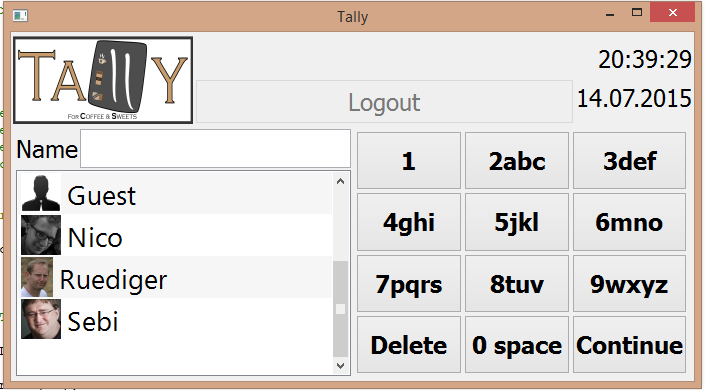
\includegraphics[width=9cm]{2Login-Screen.png}}
	\caption{Login Screen}
	\end{figure}
	
	\par
		1 : Es wird der Passwort-Screen auf dem Bildschirm angezeigt.
			Exitcode:
\begin{enumerate}			
			\item	20 : Es wurde auf den `Back' Knopf gedrückt gelangt in Zustand 0.
			\item	21 : Das Passwort wurde korrekt eingegeben und man gelangt zum Coffee/Sweet/Scan Menü.
				!20 \& !21 \& !100 \& !34 : Das Programm beendet sich.
\end{enumerate}		
\begin{figure}[h]
	\makebox[\textwidth]{
	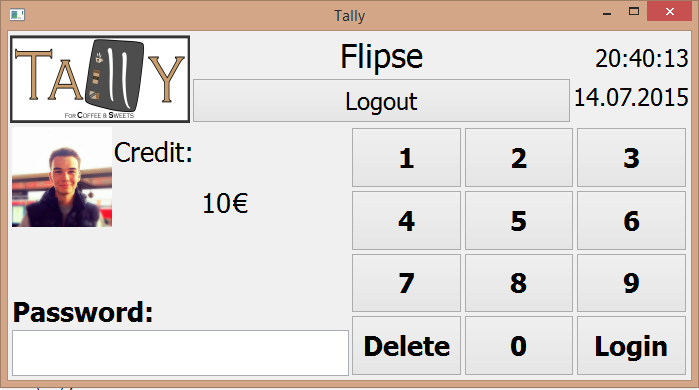
\includegraphics[width=9cm]{3Passwort-Screen.png}}
	\caption{Passwort Screen}
	\end{figure}	
\newpage
		2 : Es gibt die Auswahlpunkte zwischen Coffee/Sweets/Scan als auch die Favoriten oder das Shoppingcart.
			Exitcode:
\begin{enumerate}			
			\item	31 : Es wurde auf `Coffee' geklickt und man gelangt zur Getränkeliste mit dem Shoppingcart.
			\item	32 : Es wurde auf `Sweets' geklickt und man gelangt zur Süßigkeitenliste mit dem Shoppingcart.
			\item	34 : Es wurde ein Artikel gescannt und wird in das Scan\_Menue geleitet mit dem Shoppingcart.
			\item	35 : Es wurde auf `Favoriten' geklickt und man gelangt in den Favoriten-Screen.
			\item	36 : Es wurde auf `Settings' geklickt und wird in das Settingsmenue geschickt.
			\item	51 : Es wurde auf `Back' geklickt und man wird automatisch ausgeloggt.
			\item	99 : Es wurde auf `Buy' geklickt. Der Kaufvorgang wird beendet. Die Datenbank wird aktgualisiert und man wird in den afterbuyscreen geschickt nach einigen 						Sekunden dann wieder in den Login-Screen.
				!31 \& !32 \& !33 ! \& !34 \& !99 \& !100 \& !98 : Das Programm beendet sich.
\end{enumerate}	
\newpage
\begin{figure}[h]
	\makebox[\textwidth]{
	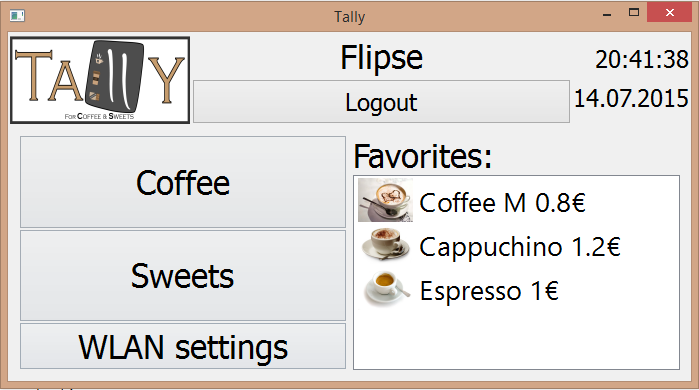
\includegraphics[width=9cm]{4CoffeeSweetsScan-Screen.png}}
	\caption{Item Screen}
	\end{figure}		
		3 : Es wird die Getränkeliste mit dem Shoppingcart gezeigt.
			Exitcode:
\begin{enumerate}			
			\item	51 : Es wurde auf `Back' geklickt und man wird in Zustand 2 gesetzt.
			\item	99 : Es wurde auf `Buy' geklickt. Der Kaufvorgang wird beendet. Die Datenbank wird aktgualisiert und man wird in den afterbuyscreen geschickt nach einigen 						Sekunden dann wieder in den Login-Screen.
			\item	98 : Ein Artikel wurde aus dem Warenkorb entfernt und wird wieder in der Getränkeliste aufgelistet.
\end{enumerate}
\begin{figure}[h]
	\makebox[\textwidth]{
	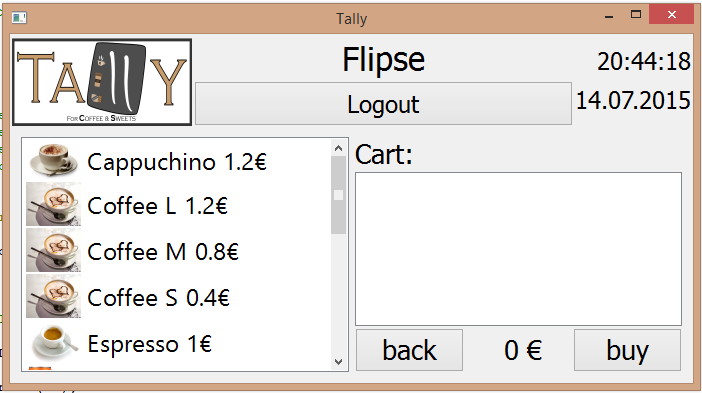
\includegraphics[width=9cm]{5CoffeList-Screen.png}}
	\caption{Coffe + Cart Screen}
	\end{figure}			
		4 : Es wird die Süßigkeitenliste mit dem Shoppingcart gezeigt. 
			Exitcode:
\begin{enumerate}			
			\item	51 : Es wurde auf `Back' geklickt und man wird in Zustand 2 gesetzt.
			\item	99 : Es wurde auf `Buy' geklickt. Der Kaufvorgang wird beendet. Die Datenbank wird aktgualisiert und man wird in den afterbuyscreen geschickt nach einigen 						Sekunden dann wieder in den Login-Screen.
			\item	98 : Ein Artikel wurde aus dem Warenkorb entfernt und wird wieder in der Süßigkeitenliste angezeigt.
\end{enumerate}	
\begin{figure}[h]
	\makebox[\textwidth]{
	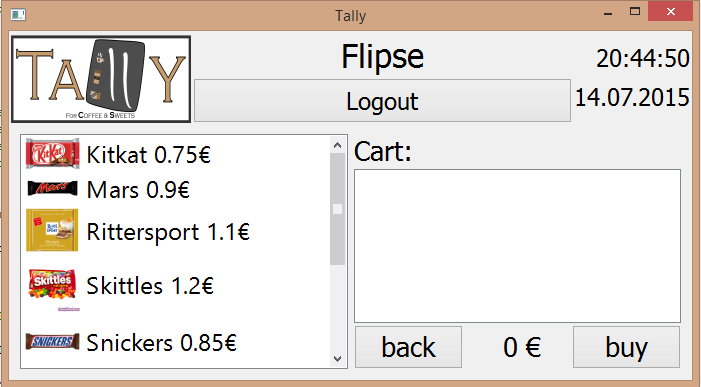
\includegraphics[width=9cm]{6SweetsList-Screen.png}}
	\caption{Login Screen}
	\end{figure}		
		5 : Es wird das Scan-Menue angezeigt.
\begin{enumerate}		
			\item	51 : Es wurde auf `Back' geklickt und man wird in Zustand 2 gesetzt.
			\item	99 : Es wurde auf `Buy' geklickt. Der Kaufvorgang wird beendet. Die Datenbank wird aktgualisiert und man wird in den afterbuyscreen geschickt nach einigen 						Sekunden dann wieder in den Login-Screen.
\end{enumerate}		
\begin{figure}[h]
	\makebox[\textwidth]{
	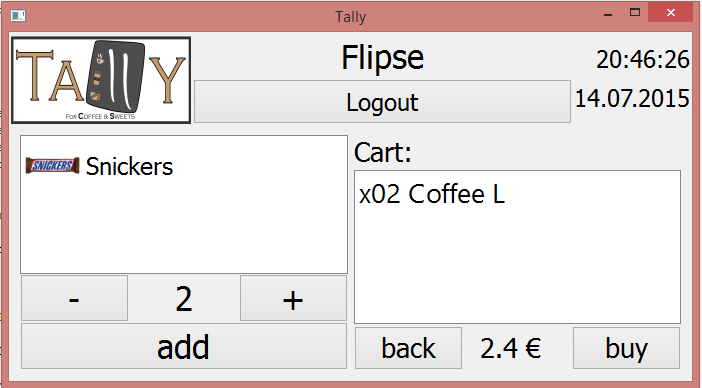
\includegraphics[width=9cm]{8Scan-Screen.png}}
	\caption{Scan Screen}
	\end{figure}
	\newpage
		6 : Es wird das Shoppingcart als auch die Favoriten angezeigt.
\begin{enumerate}		
			\item	99 : Es wurde auf `Buy' geklickt. Der Kaufvorgang wird beendet. Die Datenbank wird aktgualisiert und man wird in den afterbuyscreen geschickt nach einigen 						Sekunden dann wieder in den Login-Screen.
			\item	51 : Es wurde auf `Back' geklickt und man wird in Zustand 2 gesetzt.
			\item	98 : Ein Artikel wurde aus dem Warenkorb entfernt und wird wieder in der Favoritenliste angezeigt.
\end{enumerate}				
		7 : Es werden die Settings angezeigt(Nur als Admin)
\begin{enumerate}		
			\item	71 : Es wurde auf `Back' geklickt und man wird in Zustand 2 gesetzt.
\end{enumerate}
\begin{figure}[h]
	\makebox[\textwidth]{
	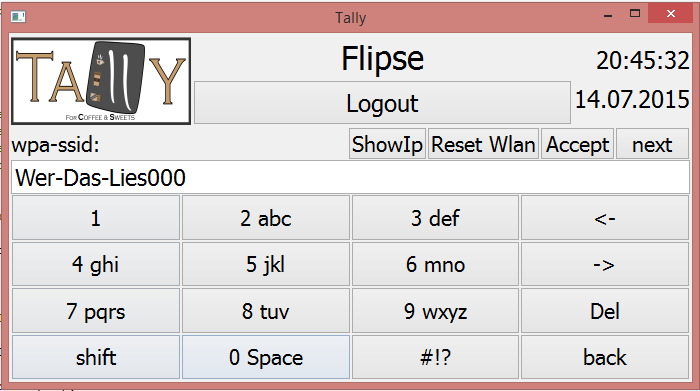
\includegraphics[width=9cm]{7Settings-Screen.png}}
	\caption{Settings Screen}
	\end{figure}

\paragraph{mainwindows.cpp:} $\;$ \\
	Wie bereits erwähnt haben wir die Oberfläche in zwei Teile unterteilt, in welche dann Widget hinzugefügt und entfertn werden können. 
	Für diese Unterteilung ist die mainwindow.cpp verantwortlich, als auch noch für andere Funktionen.-->(BILD1)<--
	Die Kopfzeile wird erzeugt und dann nur noch verändert, bezüglich Datum,Zeit,Name und ob der Logout-Button aktiv ist.
	Der Automatenbereich wird mit jedem Zustanswechsel verändert.
	Durch die Funktion 
	\begin{frame}

\begin{lstlisting}
-->removeWidget()
\end{lstlisting}
\end{frame}
werden alle Widgets die sich im Automatenbereich befindet entfernt, wodurch neue Widget dort gesetzt werden können.
	Fast jeder Screen besitzt eine Funktion names setMainWindowPointer. In diesem wird der Bezug zwischen dem Screen und dem mainwindow hergestellt.
	Außerdem wird dieser Funktion auch die User\_Id mitübergeben, damit in der Klasse die User\_id des angemeldeten Benutzers bekannt ist.
	\begin{frame}

\begin{lstlisting}
	setMainWindowPointer(QApplication *a,QString gUserId)
	\end{lstlisting}
\end{frame}
	
	Alle Funktionen die mit 
	\begin{frame}

\begin{lstlisting}
	show
	\end{lstlisting}
\end{frame}
	beginnen, sind dafür da die entsprechenden Widget in dem Fenster zu erstmalig zu zeigen.
	Die Funktionen die mit 
	\begin{frame}

\begin{lstlisting}
	update
	\end{lstlisting}
\end{frame}
	beginnen, updaten die entsprechend Widgets um auf entsprechende Events zu reagieren.
	Im Konstruktor der Klasse wird erstmalig die Uhrzeit und das Datum ermittelt. Dies funktioniert über die von Qt zur verfügung gestellten Klassen QTime und QDate.
	Diese Funktionen ermitteln die aktuelle Zeiten über das Betreibssystem, über welches Qt momentan läuft und gibt dieses in einem, vom Programmierer gewählten Format, zurück.
	
	\begin{frame}

\begin{lstlisting}
	QTime qtime = QTime::currentTime();
	QString stime = qtime.toString(Qt::LocalDate);
	\end{lstlisting}
\end{frame}
	Zusätzlich bietet QTime noch die Funktion 
	\begin{frame}

\begin{lstlisting}
	timerEvent(QTimerEvent *event)
	\end{lstlisting}
\end{frame}
	Diese Funktion wird jede Sekunde ausgeführt. Dadurch wird ein Zähler erzeugt denn wir für mehrere Funktionen genutzt haben.
	Einerseits wird die Zeit jede Sekunde aktualisiert um die aktuelle Uhrzeit auf der Oberfläche anzeigen zu lassen.
	Andererseits nutzten wir den Zähler auch für den Watchdog. Diese wird jede Sekunde einen hochgesetzt. Wenn eine gewisse Anzahl, welche in den Setting(Datenbank) angegeben ist, erreicht, 
	wird der Benutzer automatisch abgemeldet und man landet wider in dem Login-Screen. Bei jedem Tastendruck, unabhängig in welchem Screen man sich befindet, wird der Watchdog wieder zurückgestellt.
\par	
	Zusätzlich wird auch die, von Qt zur Verfügung gestellt Klasse QKeyEvent verwendet. In der Funktion 
	\begin{frame}

\begin{lstlisting}
	keyPressEvent(QKeyEvent *ev)
	\end{lstlisting}
\end{frame}
	  wird ein Tastendruck der Tastur erfasst und wird an einen String angehangen.
	Sobald `Enter' gedrückt ist, wird ein Exitcode geworfen. Diese Funktion realisiert den Barcode-Scanner. 
	Das Signals des Barcode\_Scanners verhält sich wie ein Signal von der Tastatur und beendet den eingelesen Code mit einem `Enter'. Mit dieser Funktion ist der Barcode\_scanner implementiert.
\par	
\paragraph{loginscreen.cpp:} $\;$ \\
	Im Login-Screen werden auf der Linken Seite alle Benutzer aufgelistet die in der Datenbank vorhanden sind. Dies geschieht über eine QListWidget in welche QListWidgetItem's hinzugefügt wird.
	In den QListWidgetItem's werden die Werte der Benutzer gespeichert, wlche über die Datenbank eingefortdert wurden. 
	\begin{frame}

\begin{lstlisting}
	QListWidgetItem *item = new QListWidgetItem();      //Erzeugen eines Benutzers
       item->setData(4,Database.getString(0).toInt());     //User\_Id wird an vierter Position gespeichert
       item->setIcon(Database.getPixmap(3));               //Bild des Benutzers wird gespeichert
       item->setText(Database.getString(2));               //Nickname des Benutzers wird gespeichert
       ui->listWidget->addItem(item);                      //Neuer Benutzer wird in die Tabelle hinzugef\''ugt
       \end{lstlisting}
\end{frame}
\par
	Auf der rechten Seite erscheint eine Tastatur. Auf den 8 Knöpfen verteilt stehen die Buchstaben des Alpabhets. Jeweils 3 oder 4 Buchstaben pro Knopf.
	Nun kann man seinen Account in der Liste suchen. Entweder man scrollt in der Liste so lange bis man sich gefunden hat oder man gibt seinen Namen, rechts auf der Tastatur ein.
	Auf der Tastatur muss man seinem Namen mithilfe seines T9 Codes eingeben. Dies bedeuted jeder Buchstabe in seinem Namen wird durch eine Zahl ersetzt(Zahl laut Tastatur), 
	wodurch die Namen auf der rechten Seite verschwinden, die keine Teil des bisher Eingegebenen Codes sind.
	Realisiert haben wir dies, indem von jedem Benutzer der T9\_Code in der Datenbank gespeichert ist und nun mitHilfe des compare()Befehls von QString verglichen wird.
	\begin{frame}

\begin{lstlisting}
	if(tempID.contains(NameField) || NameField.length() == 0){      //vergleicht den eingegeben Code(Namefield) mit den Werten aus der Datenbank  
	\end{lstlisting}
\end{frame}
\par	
	Wenn der Benutzer seinen Account gefunden hat kann er auf diesen klicken und gelangt automatisch in denn Passwort-Screen.
	Auserdem wird bei diesem Befehl, die User\_Id gespeichert, womit andere Funktionen wissen welcher Bemnutzer sich anmelden möchte.	
\par
\paragraph{passwordscreen.cpp:} $\;$ \\
	Im PasswordScreen erscheint auf der linken Seite, das Bild als auch der Credit des Benutzers. Auf der Rechten Seite befindet sich eine Tastatur mit den Zahlen von 0 bis 9, wodmit der Benutzer sich anmelden kann.
	Wenn der Benutzer sein Passwort korrekt eingegeben hat, wird bei der Datenbankabfrage bezüglich Benutzer und Passwort , den Wert true zurückgeben und man wird automatisch in den den Coffee/Sweet/Scan -Screen weitergeleitet.
	\begin{frame}

\begin{lstlisting}
	if(database.checkPassword(userId,password) \&\& blocked != `1' \&\& database.checkUserLoginCount(userId)){  //Passwort wurde korrekt eingegeben und der User ist niocht geblockt
            database.updateLoginAttempt(userId,true);
            Data.close();
            mainWindowPointer->exit(21);<--
            \end{lstlisting}
\end{frame}
\par			
	Außerdem wurde der Zeitstempel für den User gesetzt. 
	Falls sich der Benutzer drei mal mit dem Falschen Passwort anmelden wollte wird dieser Account für 60 Sekunden geblocket.
	Dies geschieht in dem wir, bei den letzten misslungten einloggen den Zeitstempel speichern und einen Zähler erhöhen(beide Werte werden in der Datenbank gespeichert).
	Nun wird bei jedem misslungenen einloggen der Zähler erhöht. Wenn dieser die drei erreicht, wird der account für 60 Sekunden gespeert.
	Sobald man sich einmal richtig einloggt wird der Zeitstempel aktualisiert und der Zähler wider auf 0 gesetzt. Die Funktion für die Datenbankänderung gibt die Klasse sqlzugriff, wobei die Abfrage über eine if-Anweisung geklärt wird.
	
	\begin{frame}

\begin{lstlisting}
if(database.checkPassword(userName,password))
\end{lstlisting}
\end{frame}
\par	
	Falls der Benutzer gesperrt ist, wird anstelle des Credits, die Nachricht angezeigt `User blocked' angezeigt.
	
	\begin{frame}

\begin{lstlisting}
	ui->label\_name->setText(`User blocked');
	\end{lstlisting}
\end{frame}
	Falls der Benutzer nur kurzeitig gespeert ist aufgrund zu häufiger Eingabe des falschen Passwortes, wird dieser auch geblockt.
	Dann erscheint ansttele des Credits `Wrong login!' und `Temp blocked.'
	Es wird eine Loginversuch immer dann als gescheitert definiert, wenn der Benutzer Login drückt und ein falsches Passwort eingegeben wurde und dann, wenn auf delete gedrückt wurde.
\par	
\paragraph{favwidget.cpp :} $\;$ \\
	Diese Klasse beinhaltet den Screen der Favoriten.Diese enthält die Funktion setMainWindowPointer wodurch es die Schnittstelle liefert zwischen mainwindow.cpp und der favcart.cpp.
\par
\paragraph{favcart.cpp \& buywidget.cpp:} $\;$ \\	
	favcart.cpp zeigt die Favoriten an des jeweiligen Benutzers. buywidget.cpp zeigt entweder die Getränkeliste oder die Süßigkeitenlsite an.
	Welcher der beiden Liste gezeigt wird, wird dem der Funktion über die setMainwindowPointer Funktion bekanntgegeben.
	
	\begin{frame}

\begin{lstlisting}
	setMainWindowPointer(QApplication *a,QList<QListWidgetItem> *cartItems,bool gSweetsActive,QString gUserId)
	\end{lstlisting}
\end{frame}
	Wenn der bool Wert true ist wird die Süßigkeitenliste angezeigt, andernfalls die Getränkeliste. Die Werte dafür werden jeweils aus der Datenbank gezogen.
\par	
	Beiden Klassen sind gleich Aufgebaut. Sie besitzen ein Tabelle wo alle Artikel aufgelistet sind. Dies wird über eine QListWidget organisiert wie bereits die Namen im Login-Screen.
	In den QListWidgetItem's sind folgende Werte an deren Position gespeichert:
	
	\begin{frame}

\begin{lstlisting}
	- Der Name der Artikels wird der Name des QListWidgetItem's (item->setText(name);)
	- Das Bild des Artikels hat einen extra Platz im QListWidgetItem (item->setIcon(picture);)
	- An der vierten Stelle wird die Artikel ID gespeichert (item->setData(4,itmeID);)
	- An der f\''unften Stelle wird der Preis des Artikels gespeichert (item->setData(5,price);)
	- An der sechsten Stelle wird die Menge gespeichert die noch vorr\''atig ist (item->setData(5,amount);)
	\end{lstlisting}
\end{frame}
\par
	An den ersten drei Stellen sind wir uns nicht sicher was dort gespeichert wird.
	Wir können nichts darauf expliziet speichern und wenn wir ausgeben lassen was dort gespeichert ist, bekommen wir einen leeren String zurück.
\par	
	Zusätzlich verändert sich die Farbe bei unterscheidlichen Beständen. Bei nur noch einem vorhanden Element wird der Name Rot angezeigt und bei unter 6 Elementen ändert sich die Farbe des Testes auf Gelb.
\par	
\paragraph{coffeesweetsscan.cpp :} $\;$ \\
	In diesem Screen hat an die Möglichkeit zu wählen, zwischen der Getränkeliste und der Süßigkeitenliste. Gegebenenfalls bei Adminrechte auch den Button für die Settings.
	Diese Auswahlmoglichkeiten stehen auf der Rechten Seite und können durch anklicken ausgewählt werden. 
	Auf der linken Seite befindet sich entweder das Shoppingcart, falls in diesem Items liegen oder falls das Shoppingcart leer ist, steht dort die Favoriten.
\par	
\paragraph{shoppingcart.cpp :} $\;$ \\
	Das shoppingcart ist verantwortlich für den eigentlichen kauf. Es kombinbiert die Einkäufe aus den beiden Einkaufslisten, den eingescannten Artikeln und die aus dem Favoriten.
	Das Shoppingcart selber ist wider eine QListWidget mit QListWidgetItem's, wie bereits mehrmals verwendet.
	Mit der Funktion 
		\begin{frame}

\begin{lstlisting}
	-->void Shoppingcart::updatePrice()
	    \end{lstlisting}
\end{frame}
	 wird der Preis aller Artikel im Shoppingcart aktualisiert. 
	\begin{frame}

\begin{lstlisting}
	while(ui->listWidget->item(loop) != NULL){
       tempItem = ui->listWidget->item(loop);
       price = price + (tempItem->data(5).toDouble() * tempItem->data(6).toInt());
       loop++;
    }
    \end{lstlisting}
\end{frame}
	Falls der angemeldete Account nicht genügend Guthaben zur Verfügung steht wird der Preis rot markiert und es kann auch nicht eingekauft werden.
	Guthaben wird über die Datenbank ermittelt und in der Settings-Tabelle der Datenbank steht die Information um wie viel man sein Konto überziehen darf.
	Dies geschieht über die Funktion
	 \begin{frame}

\begin{lstlisting}
	bool Shoppingcart::hasEnoughCredit(QString userId,double price)
		\end{lstlisting}
\end{frame}
	Über die Funktion 
	\begin{frame}

\begin{lstlisting}
	void Shoppingcart::addItem(QListWidgetItem *item)
		\end{lstlisting}
\end{frame}
	 wird ein Item in das Shoppingcart hinzugefügt.Außerdem wird Anzahl an ausgewählten Artikel auch in den Liste verringern.
	Dadurch synchonisieren sich die Listen, wodurch nicht mehr Artikel existieren als es eigentlich gibt.
	Die Funktion
	\begin{frame}

\begin{lstlisting}
	void Shoppingcart::on\_pushButton\_buy\_clicked()(Eingabe)<--
	\end{lstlisting}
\end{frame}
	    wickelt die kaufabwicklung ab. Diese öffnet die Datenbank. ändert den Credit des Benutzers
	    
	\begin{frame}

\begin{lstlisting}
	Database.updateCredits(userId,QString::number(credits.toDouble()-price));
	\end{lstlisting}
\end{frame}
	Außerdem reduziert es die Artikelmenge in der Datenbank um die Anzahl, wie viele gekauft wurden und trägt die Käufe in den ConsumIndex-Tabelle, als auch in die Sell-History ein.
	\begin{frame}

\begin{lstlisting}
	Database.updateAmount(tempItem->data(4).toString(),QString::number(Database.getString(0).toInt() - tempItem->data(6).toInt()));
	   Database.addSell(userId,tempItem->data(4).toString(),tempItem->data(6).toString(),tempItem->data(5).toString());
       Database.updateConsumeIndex(userId,tempItem->data(4).toString(),tempItem->data(6).toString());
       \end{lstlisting}
\end{frame}
\par	   
\paragraph{scanwidget.cpp :} $\;$ \\
	Das Klasse wird erzeugt sobald ein Artikel eingescannt wurde, währrend man in Zustand 2 sich befindet.
	Bei dieser MainWindowPointer Funktion wird noch zusätzlich der eingescannte Artikel, bereits als QListWidgetItem, mit übergeben, als auch das Shoppingcart.
	Der Eingescannte Artikel erscheit auf der linken Seite in einem QListWidget, wähhrend auf der rechten Seite das Shoppingcart angezeigt wird.
	Durch die Funktionen -->void ScanWidget::on\_pushButton\_plus\_clicked() und -->void ScanWidget::on\_pushButton\_minus\_clicked() wird die Anzahl des Artikel erhöht bzz verringert.
	Durch die Funktion 
	\begin{frame}

\begin{lstlisting}
void ScanWidget::updateAmountEveryItem()
\end{lstlisting}
\end{frame}
wird die Farbe des Artikels geändert wie bereits zuvor in den Liste erwähnt.
	Durch die Funktion 
	\begin{frame}

\begin{lstlisting}
	void ScanWidget::on\_pushButton\_add\_clicked()
	\end{lstlisting}
\end{frame}
	  wir der eingescannte Artikel in das Shoppigcart hinzugefügt.
	\begin{frame}

\begin{lstlisting}
	ui->listWidget->item(0)->setText(ui->listWidget->item(0)->text().insert(0,x0 + QString::number(count) +  ));	
	\end{lstlisting}
\end{frame}
\par		
\paragraph{sqlzugriff.cpp :} $\;$ \\
	Diese Klasse ist verantwortlich für die Datenbankzugriffe.
	Ein Zugriff funktioniert wie folgt:
	Man erzeugt zuerst eine Schlange vom Typ QSqlQuery . In diese werden später die gefunden Elemente aus der Datenbank gespeichert. Nun kann man mit der Funktion .exec auf bestimmte Teile der Datenbank zugreifen.
	\begin{frame}

\begin{lstlisting}
QSqlQuery query;
	query.exec(`SELECT Value from Settings WHERE Setting\_ID = `3');
	\end{lstlisting}
\end{frame}
	An der Stelle wo im Beispiel Settings steht, kommt der Name der Tabelle geschrieben, in welcher man suchen möchte.
	An der Stelle wo im Beispiel Value steht, kommt der Spaltenname geschrieben, welchen man suchen möchte.
	An der Stelle wo im Beispiel Setting\_ID = `3' steht, steht eine Bedingung die die gesuchten Werte erfüllebn muss. Dieser Befehl muss nicht geschrieben wenn keine Bedingung vorhanden ist.
	
	\begin{frame}

\begin{lstlisting}
	picPath = query.value(0);
	\end{lstlisting}
\end{frame}
	Mit diesem Befehl, speichert man ein Element, welches in der Datenbank gefunden wurde. Falls es mehrer Werte geben sollte, benutzt man die Funktion -->query.next()
	Falls es ein nächstes Element existiert, wird das erste Elemnt der Schlange entfernt, wodurch das Element als nächstes ausgewertet werden kann. Falls kein Elemt mehr vorhanden ist, gibt die Funktion FALSE zurück.
\par	
	Außerdem kann die Klasse auch in Datenbank schreiben. Einamla kann eine neue Splate erzeugt werden durch
	
	\begin{frame}

\begin{lstlisting}
	query.exec(INSERT INTO Consum\_Index (User\_ID, Grocery\_ID, Count) VALUES(+userId+,+Grocery\_Id+,+count+));
	Zuerst wird die Tabelle mit den Spalten, die gef\''ullt werden sollen genannt Consum\_Index (User\_ID, Grocery\_ID, Count) und dann werden die einzuf\''ugenden Werte genannt (+userId+,+Grocery\_Id+,+count+).
	\end{lstlisting}
\end{frame}
\par	
	Um nun in einer Klasse auf die Datenbank zugreifen zu können, muss zuerst ein Objekt vom Typ QSqlDatabase erzeugt werden. Dann muss dem Objekt gesagt werden, das es mit einer SQL Datenbank arbeiten soll,
	auch die Stelle, an der man die Datenbank findet.
	\begin{frame}

\begin{lstlisting}
	Data = QSqlDatabase::addDatabase(QSQLITE);
	Data.setDatabaseName(C:/SQLite/database.sqlite);
	\end{lstlisting}
\end{frame}
\par	
	Letztendlich muus die Datenbank geöffnet werden durch
	\begin{frame}

\begin{lstlisting}
	Data.open();
		\end{lstlisting}
\end{frame}
	Ab nun kann man ein Objekt erzeugen von sqlzugriff und mit deren Funktionen auf die Datenbank zugreifen.
	Am Ende muss die Datenbank noch geschlossen werden durch
		\begin{frame}

\begin{lstlisting}
	Data.close();
	\end{lstlisting}
\end{frame}
\par	
\paragraph{settingswidget.cpp :} $\;$ \\
	In diesem Screen können die WLAN Einstellungen des Rapsberry Pi verändert werden. Der Admin kann dort die WLAN SSID und das Passwort über die extra dazu implementierte Tastatur GUI angeben/ändern.
	Klickt er dann auf `accept' wird ein dirty Bit gesetzt, wodurch beim Verlassen des Widgets der WLAN Treiber neu gestartet wird. 
	\begin{frame}

\begin{lstlisting}
	process.start(`sudo service networking restart');
	\end{lstlisting}
\end{frame}
\par	
\paragraph{afterbuyscreen.cpp :} $\;$ \\
	Diese Klasse wird Aufgerufen, sobald der Warenkorb gekauft wurde. Sie enthält jediglich die Eigenschaft, mehrere Sekunden ein Screen zu zeigen auf dem der Benutzer erkennen kann, das der Kauf durchgeführt wurde.
	Danach wird diese wieder gelöscht und man gelangt in den Login-Screen.

\paragraph{showipscreen.cpp :} $\;$ \\
		Diese Klasse wird nur beim Start des Programmes erzeugt. Sie dient dazu die IP-Adresse anzuzeigen.
		
		
\section{Fazit des Tally Projekts}
Die vorgegebenen Ziele konnten alle erfüllt werden. Der Raspberry besitzt alle erforderliche Hardware und Software um einen Webserver darauf laufen lassen zu können und um das Programm darauf ausführen zu können. Der Touchscreen und der Barcodescanner arbeiten auch ohne Störungen.
\par 
Auch die selbstgeschriebene Software Tally arbeitet einwandfrei und der Einkauf von Produkten funktioniert. Der Zuigriff auf die Datenbank erfolgt ebenfalls, sodass die dort gespeicherten Informationen über die Website eingesehen und geändert werden können.
\par
Probleme gab es zum Teil bei der Einrichtung von Backups auf dem Raspberry, die aber durch eine weit verbreitete Methode, rsync, behoben werden konnten. Wie zunächst gedacht konnte allerdings leider nicht das Barcodescannermodul verwendet werden, da die Spannung am Raspberry zu hoch ist, weshalb wir auf einen USB Barcodescanner umgestiegen sind.
\par
Bei der Programmierung der Website und des Tally Programmes waren die größten Probleme die Zugriffe auf die Datenbank, wie man darauf lesen und schreiben kann, und die Anordnung der einzelnen Tabellen in der Datenbank. Nach weitreichenden Recherchen konnten diese Probleme aber behoben werden.
\par
Für die Zukunft wäre es möglich einen größeren Touchscreen und ein Barcodescannermodul anzubringen. Desweiteren wäre ein Akku denkbar, sodass der Raspberyr auch bei Stromausfall noch einige Stunden arbeiten kann.
\par
Bei Tally könnte man die GUI überarbeiten. Außerdem wären weitere Einstellungsmöglichkeiten im Hauptmenü des Admins denkbar. 
\par
Auf der Website könnten noch die gewünschten Statistiken einsehbar gemacht werden.	



\newpage
\newpage
\begin{center}
\bibliographystyle{alphadin}
\bibliography{literature}
\end{center}
%------------------------------------------------------------------------------------------------

\end{document}

%------------------------------------------------------------------------------------------------